\chapter{General Information}

\section{Presentation of MS Innovative Smart System}

The \textbf{Internet of Things (IoT)} is expected to grow rapidly in the coming years. Often described as the fourth industrial revolution, IoT is a promising field, with over 20 billion smart devices projected to be connected by 2020. However, achieving this scale will involve overcoming several challenges at multiple levels. 

The \textbf{Innovative Smart Systems Master’s Program} aims to prepare young engineers to understand and tackle these challenges by developing innovative solutions. IoT systems consist of multiple layers, each with its own focus:

\begin{itemize}
    \item Perceptual Layer
    \item Network Layer
    \item Support Layer
    \item Application Layer
\end{itemize}

Each of these layers has specific challenges, addressed by different training units in the program:

\begin{itemize}
\item Designing smart devices: \textit{Smart Devices Training Unit}
\item Connecting devices: \textit{Communication Training Unit}
\item Processing data within the network: \textit{Data Processing Training Unit}
\item Providing services for network interaction and data access: \textit{Middleware and Services Training Unit}
\end{itemize}

This master’s program addresses these challenges through a variety of courses, bringing together students from diverse fields, including Electronics, Telecommunications, Computer Science, and Physics. By combining these skills, students can collaborate to solve the complex problems involved in developing IoT networks and systems.

\section{Curriculum}

\subsection{Student Profile}

\textbf{Personal information :} \\
Surname: VASSEUR.  \\
First name: Cyril.  \\
email: vasseu@insa-toulouse.fr.  \\

\subsection{Curriculum Vitae}


\noindent
\begin{minipage}{\textwidth} 
    \centering
    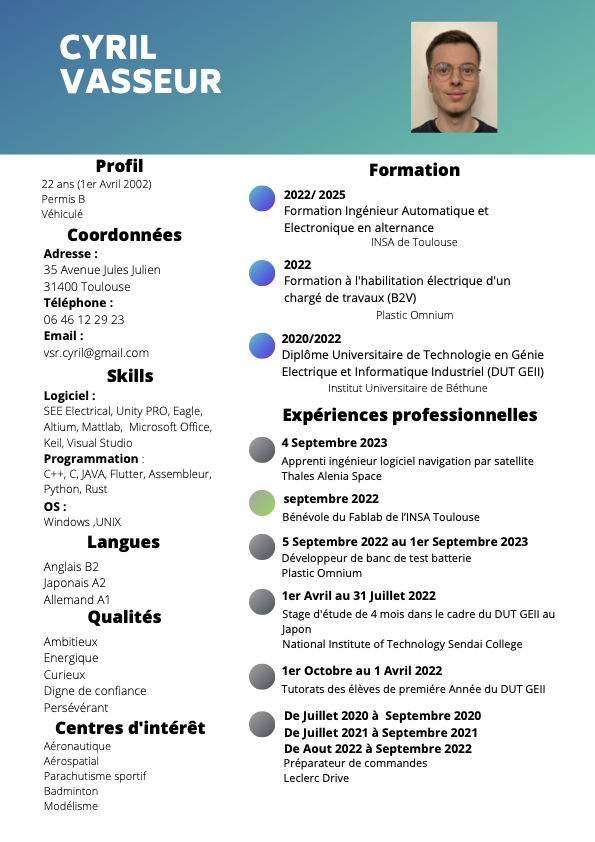
\includegraphics[width=0.8\textwidth]{image/CV_CYRIL VASSEUR.png}
    \label{fig:CV} 
\end{minipage}

\vspace{1em} 

\newpage
\subsection{Background}

Before entering INSA for my third year of higher education, I completed a two-year technical diploma (DUT) in Electrical Engineering and Industrial Computing at IUT of Béthune. 
I then pursued an engineering degree at INSA Toulouse, where I began a Master’s in Automation and Electronics through an apprenticeship program. 
My first year was spent with Plastic Omnium, where I worked on developing a test bench for heavy vehicle batteries used in trains and trucks. 
For my second year, I moved to Thales Alenia Space, drawn by my interest in the space sector, where I became a software apprentice specializing in satellite navigation.
After completing my Master’s, I continued at Thales Alenia Space to pursue my second Master’s in Innovative Smart Systems (ISS).



\subsection{Training units}

Below, you can find the overview of the various courses completed in the ISS program.

\begin{figure}[!ht]
    \centering
    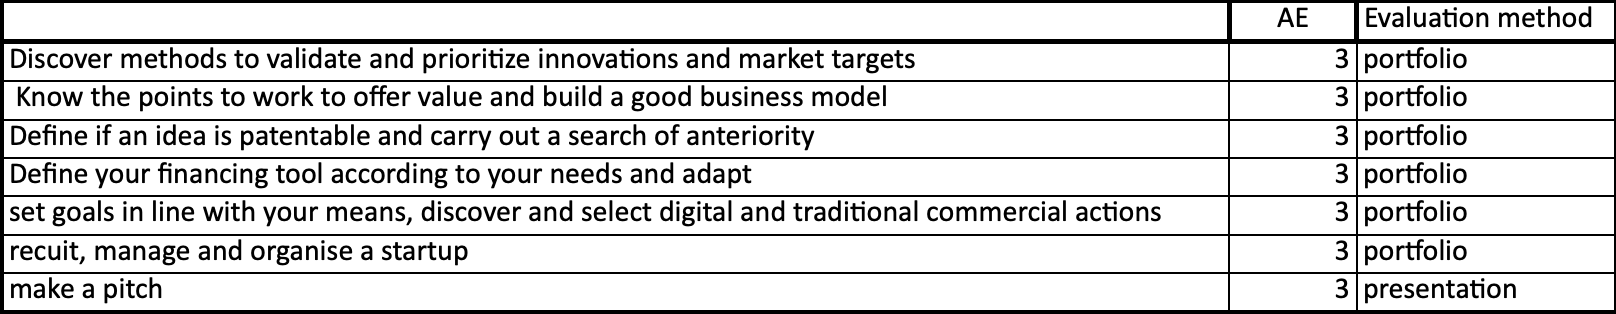
\includegraphics[width=0.8\textwidth]{image/Business startup.png}
    \caption{Business Startup Unit}
    \label{fig:Business Startup Unit}
\end{figure}
\begin{figure}[!ht]
    \centering
    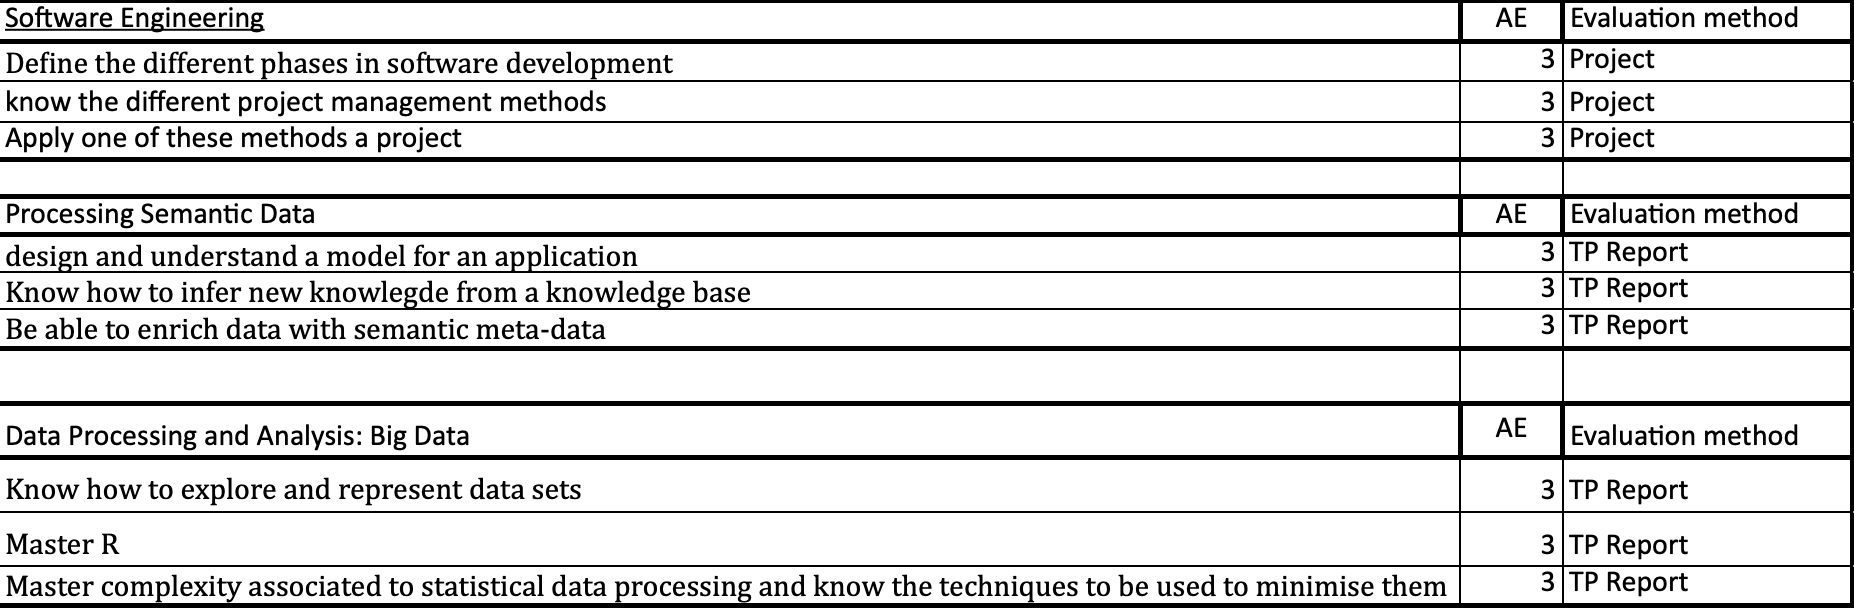
\includegraphics[width=0.8\textwidth]{image/Analysis and data processing, business applications.png}
    \caption{Analysis and data processing, business applications Unit}
    \label{fig:Analysis and data processing, business applications}
\end{figure}
\begin{figure}[!ht]
    \centering
    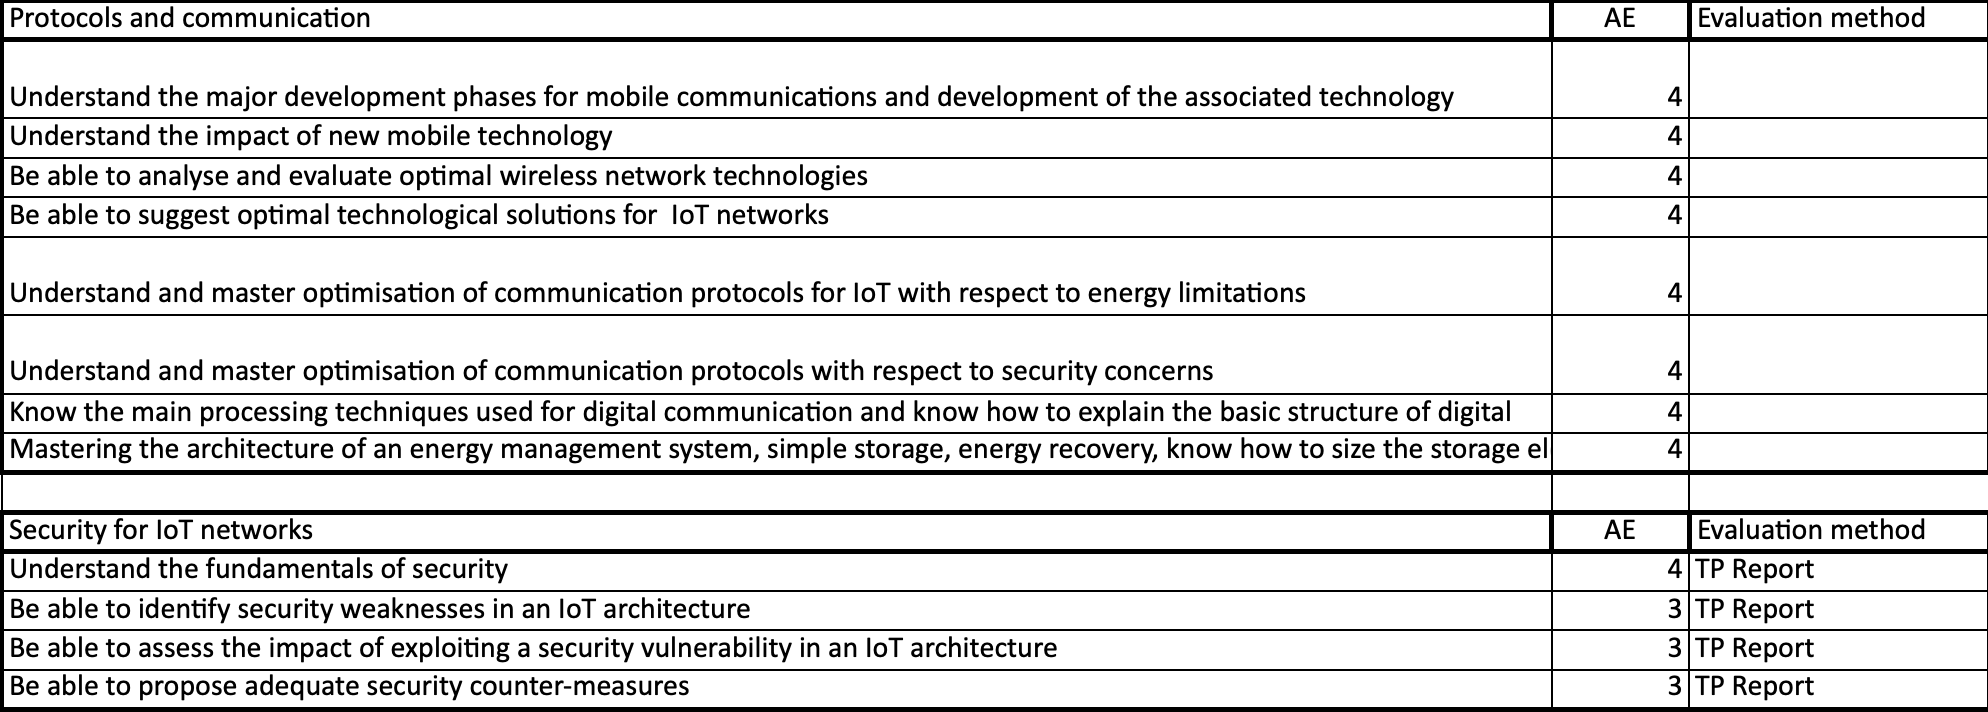
\includegraphics[width=0.8\textwidth]{image/Communication.png}
    \caption{Communication Unit}
    \label{fig:Communication}
\end{figure}
\begin{figure}[!ht]
    \centering
    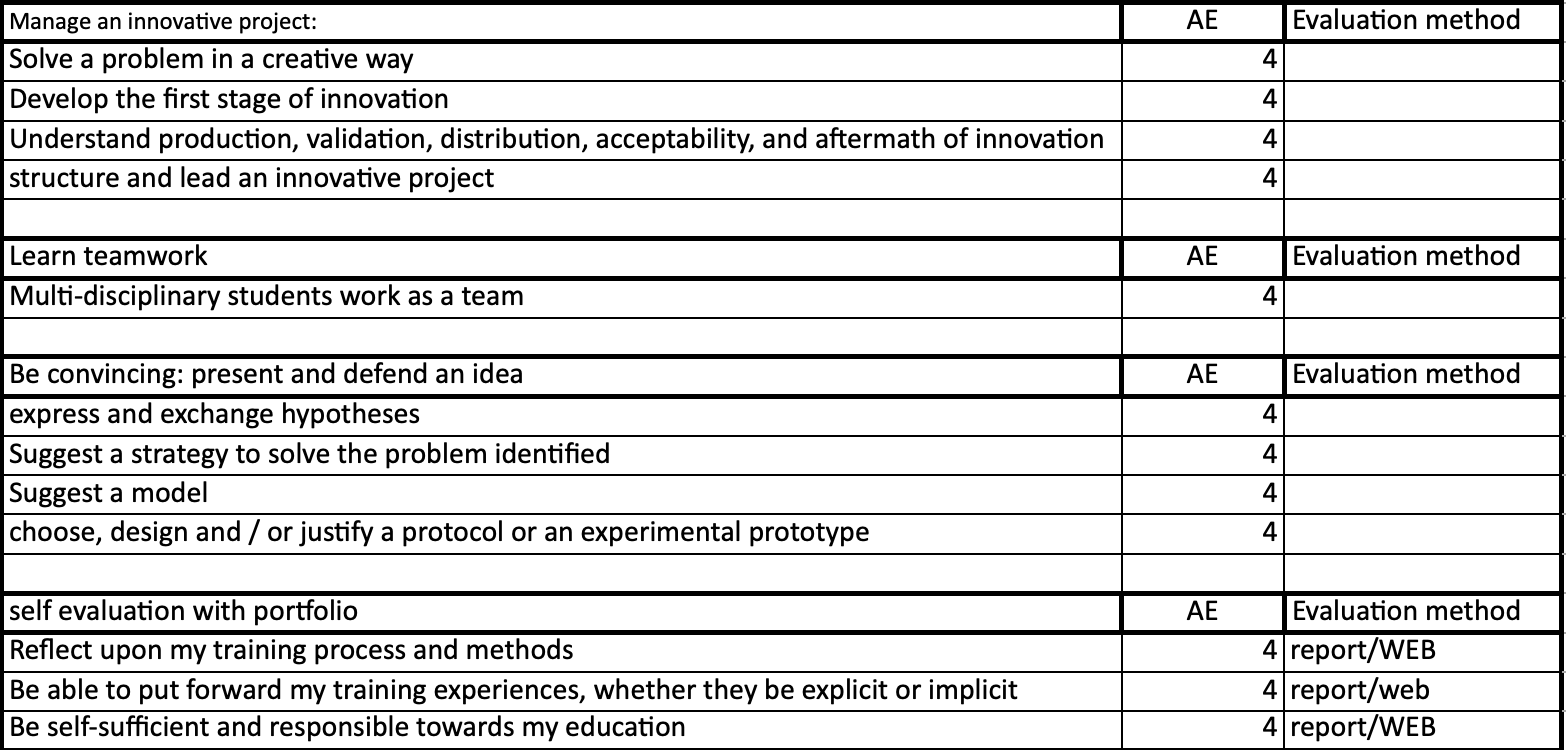
\includegraphics[width=0.8\textwidth]{image/Innovation and humanity.png}
    \caption{Innovation and humanity Unit}
    \label{fig:Innovation and humanity}
\end{figure}
\begin{figure}[!ht]
    \centering
    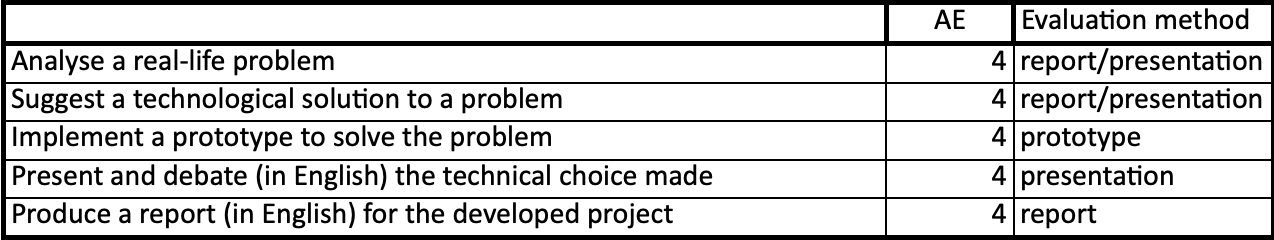
\includegraphics[width=0.8\textwidth]{image/Innovativ project.png}
    \caption{Innovative project Unit}
    \label{fig:Innovativ project}
\end{figure}
\begin{figure}[!ht]
    \centering
    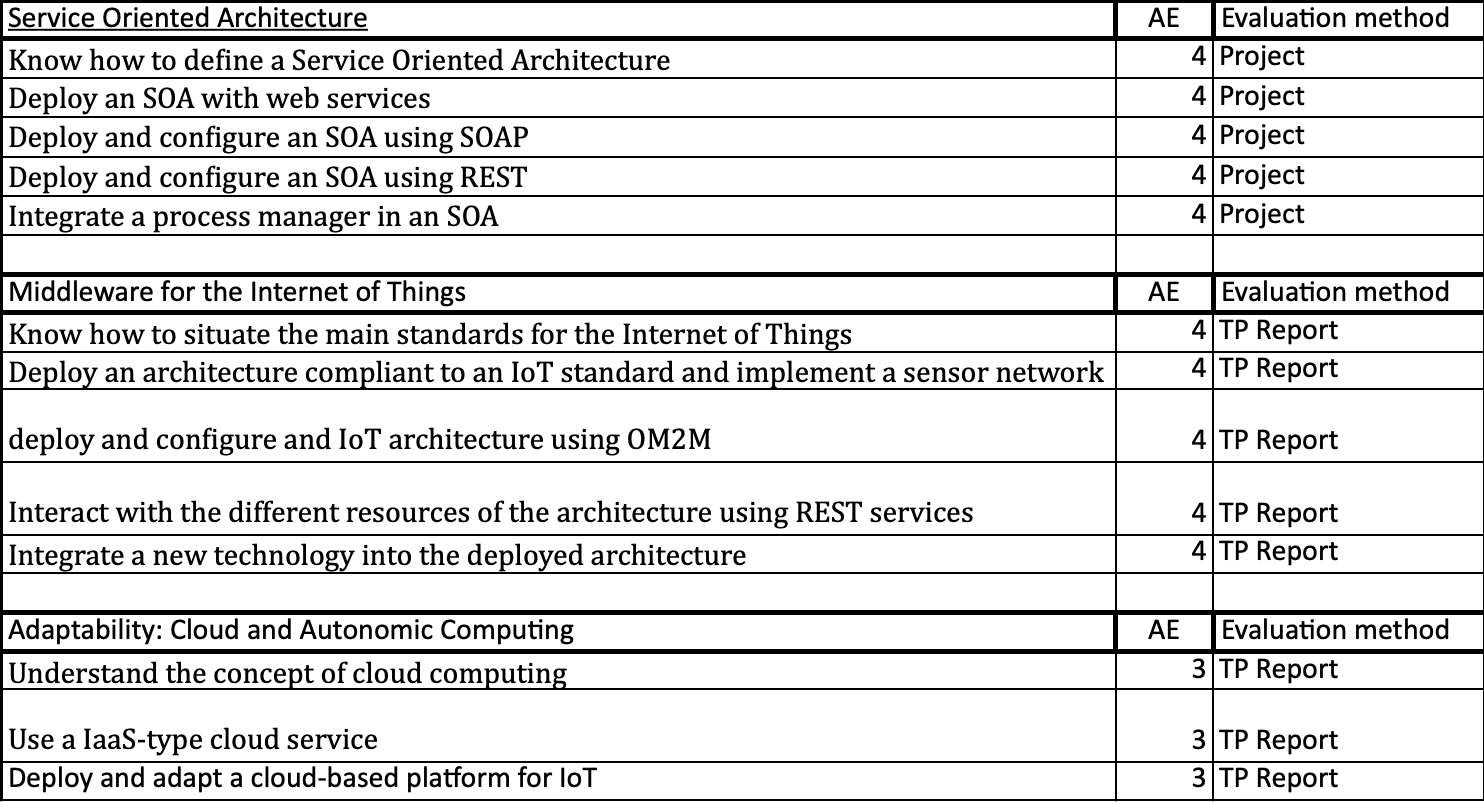
\includegraphics[width=0.8\textwidth]{image/Middleware and Service.png}
    \caption{Middleware and Service Unit}
    \label{fig:Middleware and Service}
\end{figure}
\begin{figure}[!ht]
    \centering
    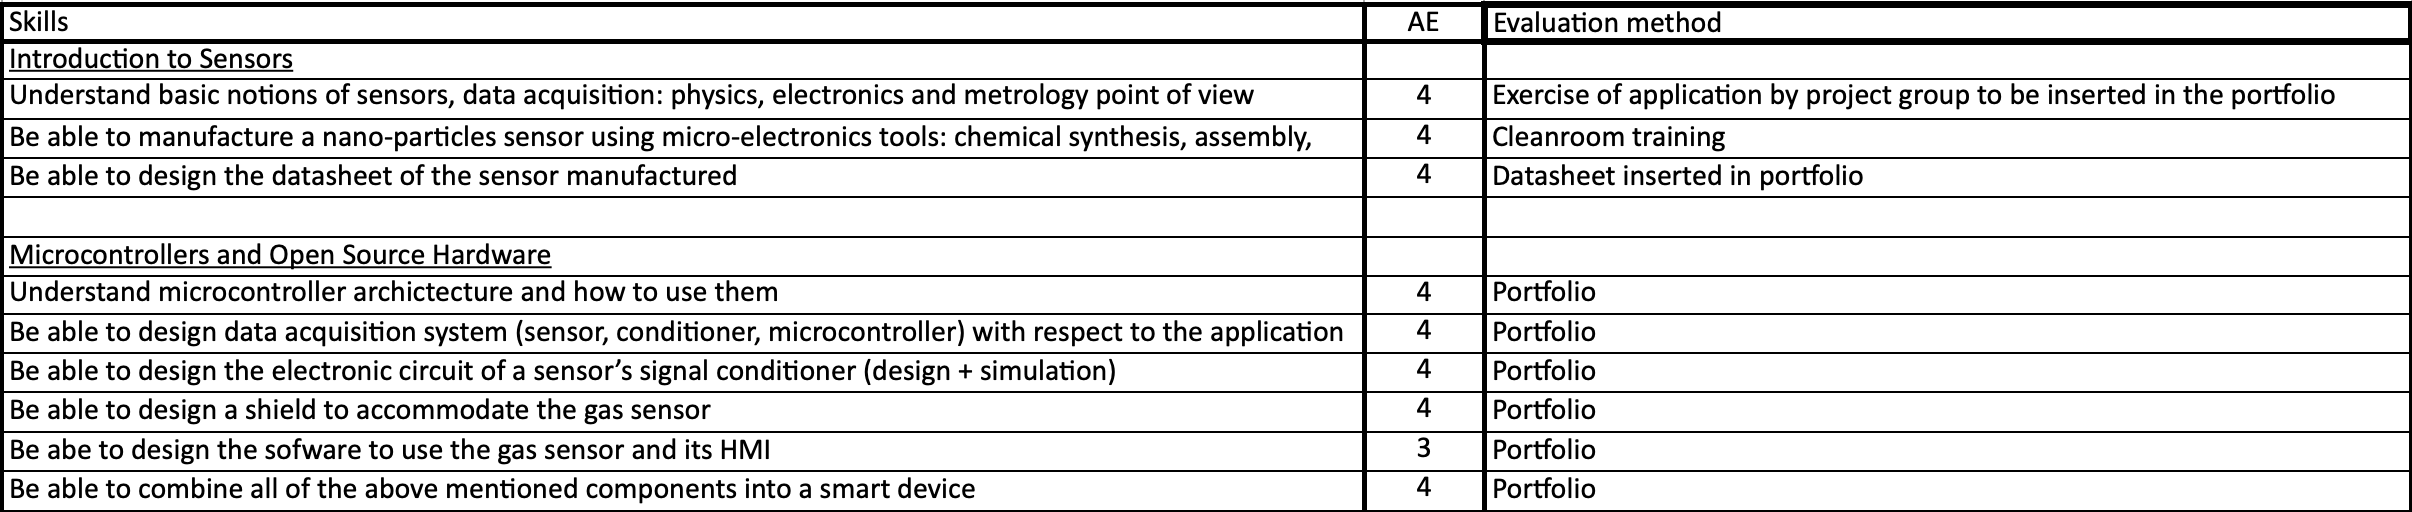
\includegraphics[width=0.8\textwidth]{image/Smart devices.png}
    \caption{Smart devices Unit}
    \label{fig:Smart devices}
\end{figure}
\newpage
\begin{figure}[H]
    \centering
    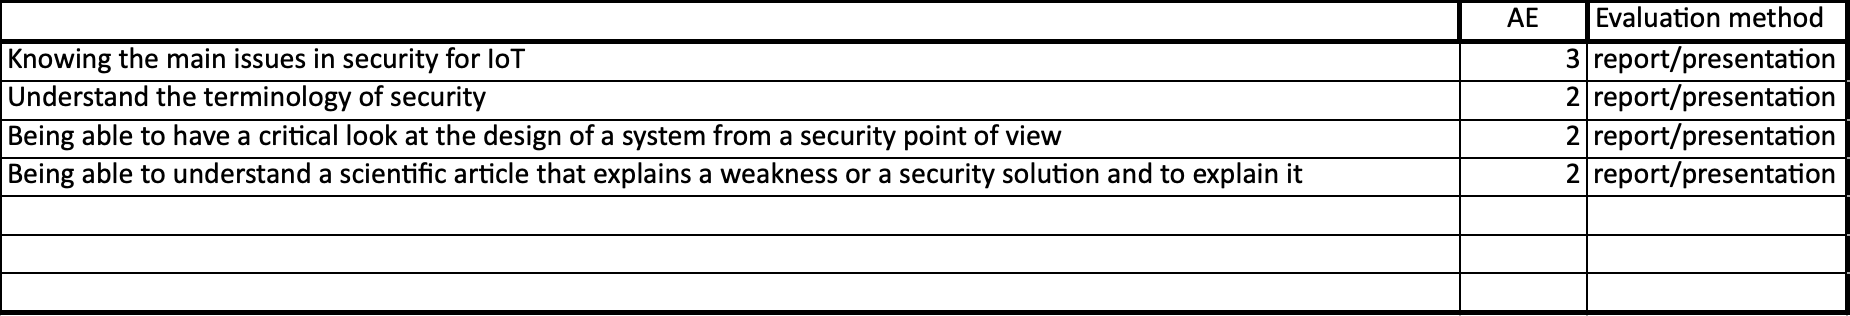
\includegraphics[width=0.8\textwidth]{image/Security.png}
    \caption{Security Unit}
    \label{fig:Security}
\end{figure}


\subsection{apprenticeship}

\subsubsection{Descriptive}